\section{Redes de comunicaciones moviles terrestres}
\subsection{Sistemas \acrshort{PMR} y \acrshort{PMT}}
\begin{itemize}
\item{\acrshort{PMR}(Private Movil Radio):} Sistemas normalmente no conectados a la red telefónica pública conmutada que se modelan como sistemas de espera.
\item{PMT(Personal Movil Telecommunications):} Sistemas conectados a la red telefónica pública modelados como sistemas con pérdidas. 
\end{itemize}
\subsubsection{Private Movil Radio}
\label{ssub:PMR}
Las características que definen este sistema son las siguientes:
\begin{itemize}
	\item Tienen una area territorial limitada.
	\item No suelen estar conectados a la red telefónica pública conmutada(POTS).
	\item Se suelen usar para dar servicios de empresa como la gestión de flotas.
	\item Deben ser posibles tanto las llamadas entre estaciones moviles (\acrshort{MS}) entre sí como las llamadas a grupos.
	\item Deben funcionar en regimen de espera con llamadas frecuentes y de corta duración.
	\item Lo normal es que funcionen en simplex pero hay casos de sistemas en semiduplex e incluso en full-duplex.
\end{itemize}
El ejemplo más representativo de los sistemas \acrshort{PMR} es el sistema Trans European Trunked RAdio (\acrshort{TETRA}). Dependiendo de como se asignen los canales de comunicación a los ususarios del sistema se puede distinguir entre los dos siguientes sistemas:
\begin{itemize}
	\item Asignación rígida: a un conjunto de ususarios se les asigna un único canal para la comunicación. Es un sistema de asignación bastante poco efectivo, por esto, se suele usar con colectivos relativamente pequeños.
	\item Asignación troncal: se tienen N canales que pueden ser usados por M usuarios.
\end{itemize}
l
\begin{example}[Sistemas PMR]
Se tiene un sistema \acrshort{PMR} en el que los usuarios piden 1 llamada de 20 segundos por \acrshort{HC}
\begin{gather*}
	\mu=\sfrac{1}{20}s^{-1}\\
	a_o=\frac{\lambda}{\mu}=\frac{20}{3600}=5.56mE	
\end{gather*}
\begin{center}
\begin{tabular}{|c|c|c|}
\hline
	N canales 	& Asignación fija 	& Asignación troncal \\\hline
	1 			& 21 				& 21 \\\hline
	2 			& 42 				& 125 \\\hline
	5 			& 105 				& 581 \\\hline
	10 			& 210 				& 1429 \\\hline
\end{tabular}
\end{center}
\begin{gather*}
0,05=C(1,A_O)e^{-\mu t(1-\rho)}=C(1,A_O)e^{-1+A_O}=A_Oe^{A_O-1} \to A_O=0,121E\\
M=\sfrac{A_O}{a}=21.7\to M=21\text{ móviles}
\end{gather*}
\end{example}
La cobertura de los sistemas \acrshort{PMR} depende de la locaclización de las estaciones base (\acrshort{BS}). En caso de que no sea necesaria una gran cobertura se utilizan sistemas monoemplazamiento. La red con cobertura monoemplazamiento está formada por un nodo central de control y su \acrshort{BS}. Una red Multiemplazamiento, en cambio, está concebida para zonas de gran extensión cubierta por varios nodos interconectados. En este esquema habrá un nodo central de control. En los sistemas multiemplazamiento \acrshort{PMR}  el traspaso no está garantizado, con lo cual, en caso de cambiar el nodo de cobertura la llamada podrá cortarse.\\
	En el siguiente esquema se pueden encontrar las unidades funcionales de un sistema \acrshort{PMR} multiemplazamiento.
\begin{itemize}
	\item 	\acrshort{BS}: Base Station
	\item 	\acrshort{CRT}: Cathode Ray Tube
	\item 	\acrshort{NMC}: Network Management Center
	\item 	\acrshort{MS}: Mobile Station
	\item 	\acrshort{TSC}: Transit Switching Center
	\item 	\acrshort{PABX}: Private Automatic Branch eXchange
	\item 	\acrshort{RTPC}: Red Telefónica Pública Conmutada
	\item 	R: Receptor
	\item 	T: Transmisor
\end{itemize}
\begin{figure}[htp]
\centering
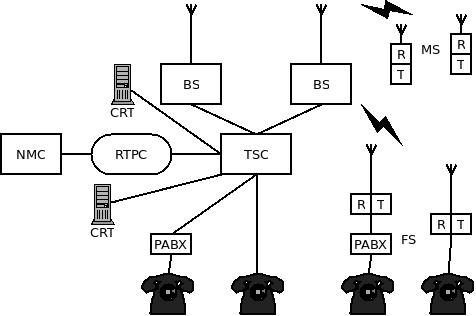
\includegraphics[width=\textwidth]{Imagen/diaPMR.jpg}
\caption{Estructura de un sistema \acrshort{PMR}  multiemplazamiento}
\label{img:diaPMR}
\end{figure}
% subsubsection PMR (end)
\subsubsection{Sistemas \acrshort{PMR}: Sistemas troncales}
\label{ssub:troncales}
	Son sistemas de concentración de enlaces, en donde la asignación de frecuencias a los usuarios es dinámica. Son sistemas en espera y se utiliza la función Erlang-C para su dimensionamiento. Por su necesidad de dinamismo es necesario un sistema de señalización para la asignación de canales y la gestión de las colas de llamadas. Para la señalización se suele utilizar un protocolo ALOHA ranurado con longitud de trama variable.\\	
% subsubsection troncales (end)
\subsubsection{Sistemas \acrshort{PMT}}
\label{ssub:PMT}
	Los objetivos de los sistemas \acrshort{PMT} son los siguientes:
\begin{itemize}
	\item Gran capacidad de abonados.
	\item Calidad telefónica igual o superior al servicio fijo.
	\item Utilización eficaz del espectro (planificación de frecuencias).
	\item Conmutación automática de radioenlaces.
	\item Capacidad de expansión.
	\item Coste razonable.
\end{itemize}
Los sistemas \acrshort{PMT} tienen una serie de conceptos muy relacionados y necesarios para la conscución de los objetivos.
\begin{itemize}
	\item Handoff, handover o traspaso: conmutación de una \acrshort{BS} a otra de una llamada en curso (que no se corte la llamada durante el cambio de cobertura de una llamada).
	\item Roaming o itinerancia: capacidad de operación de un móvil en un área de servicio distinta de aquella en la que se ha abonado inicialmente.
	\item Canal directo o descendente: canal radio para la transmisión en sentido \acrshort{BS}$\to$\acrshort{MS}. En sistemas terrestres este canal usa la mayor frecuencia disponible para que el mayor gasto energético se produzca en el \acrshort{BS} y no en el \acrshort{MS}.
	\item Canal de retorno o ascendente: canal radio para la transmisión en sentido \acrshort{MS}$\to$\acrshort{BS}. En sistemas terrestres este canal usa la menor frecuencia disponible para que el menor gasto energético se produzca en el \acrshort{MS} y no en el \acrshort{BS}.
\end{itemize}
% subsubsection PMT (end)
\subsubsection{Sistemas celulares}
\label{ssub:celulares}
	Las zona de cobertura se dividen en zonas más pequeñas llamadas celdas o células. La cobertura en estos sistemas está limitada por interferencia, es decir, por como la siguiente celda con las mismas bandas afecta a la celda. Para esto usamos el cálculo señal sobre interferencia $\sfrac{S}{I}$. La distancia de separación entre dos celdas que comparten la banda se denomina distancia cocanal o función de relación de protección. Las frecuencias disponibles se dividen en subgrupos y se asignan subgrupos a las \acrshort{BS}. Un conjunto de \acrshort{BS} que contiene todas las frecuencias disponibles se denomina agrupación o cluster. El número de celdas por cluster se identifica como J.\\
	Según las pérdidas de propagación se puede ver lo siguiente, donde D es la distancia cocanal y R es el radio de la celda:
\begin{gather*}
	I_b=kr^n\text{ pérdidas básicas de propagación.}\\
	C=\frac{P_{tx}}{kR^n}\\
	I=\frac{P_{tx}}{k(D-R)^n}\\
	\frac{C}{I}=(\frac{D-R}{R})^n\approx (\frac{D}{R})^n
\end{gather*}
Al disminuir el radio de la celda podemos ver que se puede reducir la distancia cocanal aumentando así la capacidad del sistema. Este radio se puede reducir hasta que se alcance la relación de protección $\sfrac{c}{i}_{min}$ que viene dada por las especificaciones de los sistemas.\\
Los sistemas celulares al igual que la red telefónica se modelan como sistemas con bloqueo. $p=B(N,A_o)$ siendo p la probabilidad de bloqueo, N el número de canales por celda y $A_o$ el tráfico ofrecido por los usuarios. El número de canales por célda $N=\sfrac{C}{J}$ será el número de canales disponibles al sistema entre el número de celdas por agrupación. El número de canales totales al sistema se obtendrán con el ancho de banda que se utiliza para el sistema y la separación entre radiocanales $C=\sfrac{BW}{\Delta f}$.\\
\begin{gather*}
	m=\sfrac{A_o}{a_o}\text{ número de móviles por celda}\\
	\rho_a=\frac{A_o}{S_c}\text{ Densidad de usuarios en la celda }(E/km^2)\\
	S_r=JS_c\text{ superficie de la agrupación}\\
	Q=Int(\sfrac{S}{S_r})+1\approx \sfrac{S}{JS_c}\text{ índice de reutilización}\\
	M=QJm\text{ número total de móviles en el sistema}\\
\end {gather*}
El siguiente avance radica en el uso de antenas no omnidireccionales. Las antenas omnidireccionales producen una cobertura circular que no es capaz de cubrir el plano sin solapes. Para evitar los solapes se utilizan antenas de cobertura geométrica, concretamente hexagonales, ya que tiene mayor relación aŕea-radio que los otros poligonos que pueden cubrir areas sin problemas (cuadrado y triángulo). Con el uso de celdas hexagonales además se restringe la posibilidad de agrupar las celdas a agrupaciones que sigan la serie de números rómbicos (1,3,4,7,9,12,13...).\\
La siguiente evolución de los sistemas celulares es la división o sectorización de las propias celdas dotando al sistema de mayor flexibilidad y usando antenas más direccionales. Las consecuencias de la sectorización son en su mayoría buenas. En caso de una sectorización de una celda en dos sectores, el rádio se reduce a la mitad, la superficie se divide entre cuatro y la capacidad se multiplica por cuatro. También tiene problemas, como el aumento en los costes, una mayor precisión en la colocación de las \acrshort{BS} y un aumento de la probabilidad de que haya un handoff. Con el uso de antenas direccionales se reduce además el número de antenas interferentes pudiendo aumentar la reutilización de frecuencias aumentando la capacidad del sistema.
% subsubsection celulares (end)